% -----------------------------------------------
% Modelo UFT para Trabalhos Acadêmicos
% Adaptado e mantido por Wenes (Libertário)
% Baseado no projeto abnTeX2, porém modificado para atender às diretrizes
% visuais e estruturais da Universidade Federal do Tocantins (UFT).
% Esta versão não é oficial e não substitui os modelos originais do abnTeX2.
% -----------------------------------------------
\documentclass[
	12pt,				% Tamanho da fonte
    oneside,            % Margens iguais (não alternadas)
	a4paper,			% tamanho do papel. 
	english,			% idioma adicional para hifenização
	brazilian,		    % Idioma é o principal do documento
	]{AcademicoUFT}
% -----------------------------------------------


% -----------------------------------------------
% -------------Pacotes fundamentais-------------- 
% -----------------------------------------------
\usepackage{lmodern}			% Usa a fonte Latin Modern
\usepackage[T1]{fontenc}		% Seleção de códigos de fonte.
\usepackage[utf8]{inputenc}		% Codificação do documento
\usepackage{indentfirst}		% Indenta o primeiro parágrafo
\usepackage{color}				% Controle das cores
\usepackage{graphicx}			% Inclusão de gráficos
\usepackage{microtype} 			% para melhorias de justificação
% -----------------------------------------------



% -----------------------------------------------
% FONTES
% -----------------------------------------------
\usepackage{fontspec}
%\setmainfont{XCharter}
%\setmainfont{Calibri} 
% -----------------------------------------------



% -----------------------------------------------
\usepackage{lipsum}	% para geração de texto
% -----------------------------------------------


% -----------------------------------------------
% -------------Pacotes de citações---------------
% -----------------------------------------------
\usepackage[backend=biber,style=abnt,language=brazil]{biblatex}
\addbibresource{Referencias.bib}
\usepackage{csquotes}             % Recomendado pelo biblatex 
\usepackage{etoolbox}             % Auxilia na justificação da bibliografia
\AtBeginBibliography{\justifying} % Ativa a justificação da bibliografia
\usepackage{ragged2e}
\urlstyle{same}
% -----------------------------------------------


% -----------------------------------------------
% --------VISUALIZAÇÃO E ESTABILIDADE------------
% -----------------------------------------------
\usepackage{tikz}         % Gerar imagem de exemplo
\usepackage{pgfplots}     % Funções matemática
\pgfplotsset{compat=1.18} % Garante compatibilidade
\usepackage{subcaption}   % Permite criar subfaturas
\usepackage{float}        % Adiciona a opção de posicionamento
\usepackage{amssymb}      % Necessário para símbolos matemáticos
\usepackage{amsmath}      % Necessário para comandos como \text{}
% -----------------------------------------------




% -----------------------------------------------
% -Informações para Folha de Rosto e Contracapa--
% -----------------------------------------------
\titulo{Modelo \abnTexUFT para\\ Projeto de Pesquisa por \WenesTex}
\autor{Editado por \WenesTex Aquino}
\orientador{Fulano Gomes Carvalho}
\coorientador{Beltrano Vitória Almeida}
%\supervisor{Ciclano Beatriz Santos Lima}
\local{Palmas}
\data{2025, v-1.2}

\instituicao{%
  Universidade Federal do Tocantins \\
  Campus Universitário de Palmas \\
  Curso de Licenciatura em Computação}
  
\tipotrabalho{Projeto de Pesquisa}

\preambulo{Projeto de Pesquisa apresentado como 
    parte dos requisitos para avaliação na Universidade 
    Federal do Tocantins. Este modelo foi adaptado 
    e personalizado com ajustes visuais e estruturais, 
    servindo também para testar o espaço disponível 
    utilizada nessa contracapa.}
% -----------------------------------------------


% -----------------------------------------------
\makeatletter
\hypersetup{
    colorlinks=false,  % Desativa links coloridos
    pdfborder={0 0 0}, % Remove o retângulo dos links
}
\makeatother
% -----------------------------------------------


% -----------------------------------------------
% ----------Espaçamentos e parágrafos------------ 
% -----------------------------------------------
\setlength{\parindent}{1.25cm} 
% -----------------------------------------------


% -----------------------------------------------
% ---------------Compila o Índice----------------
% -----------------------------------------------
\makeindex
% -----------------------------------------------


% -----------------------------------------------
\begin{document} % Início do documento-----------
% -----------------------------------------------
\nocite{*} % Inclui todas referências na página
\selectlanguage{brazilian}
\frenchspacing % Retira espaço extra obsoleto entre as frases.
% -----------------------------------------------


% -----------------------------------------------
% ----------FOLHA DE ROSTO E CONTRACAPA----------
% -----------------------------------------------
\imprimircapa % Está é Folha de Rosto
% -----------------------------------------------
\imprimirfolhaderosto % Esta é Contracapa
% -----------------------------------------------


% -----------------------------------------------
% -----------------ILUSTRAÇÕES-------------------
% -----------------------------------------------
\pdfbookmark[0]{\listfigurename}{lof}
\listoffigures*
\cleardoublepage
% -----------------------------------------------


% -----------------------------------------------
% ------------------TABELAS----------------------
% -----------------------------------------------
\pdfbookmark[0]{\listtablename}{lot}
\listoftables*
\cleardoublepage
% -----------------------------------------------


% -----------------------------------------------
% ------------ABREVIATURAS E SIGLAS--------------
% -----------------------------------------------
\begin{siglas}
    \item[ABNT]  Associação Brasileira de Normas Técnicas
    \item[ABNTT] Associação Brasileira de Normas Totalmente Travadas
    \item[ABNTE] Agrupamento Brasileiro de Normas Terrivelmente Escritas
    \item[ABNTX] Ajustes Básicos de Nomenclatura para Trabalhos Extraordinários
\end{siglas}
% -----------------------------------------------


% -----------------------------------------------
% ------------------ SÍMBOLOS -------------------
% -----------------------------------------------
\begin{simbolos}
    \item[$ \mathbb{N} $] Conjunto dos números naturais (Nomenclatura Padrão).
    \item[$ \Sigma $] Símbolo de Somatório ou Sigma (Usado em Análise de Dados).
    \item[$ \land $] Operador Lógico AND (Conjunção).
\end{simbolos}
% -----------------------------------------------


% -----------------------------------------------
% ------------------SUMÁRIO----------------------
% -----------------------------------------------
\pdfbookmark[0]{\contentsname}{toc}
\tableofcontents*
\cleardoublepage
% -----------------------------------------------


% -----------------------------------------------
% --------------ELEMENTOS TEXTUAIS---------------
% -----------------------------------------------
\textual


% -----------------------------------------------
% -----------------Introdução--------------------
% -----------------------------------------------
\chapter*[Introdução]{Introdução}
\addcontentsline{toc}{chapter}{INTRODUÇÃO}

\lipsum[2] \footnote{\url{http://www.latex-project.org/lppl.txt}}.
% -----------------------------------------------


% -----------------------------------------------
% -------------Capitulo de Textual---------------  
% -----------------------------------------------
\chapter{Funções Matemáticas}

\section{Morbi orci nisl hendrerit}
\lipsum[1] % Gera texto de exemplo para preencher a página. 
\cite{talbot2012}


\newpage % Nova Página 
% -----------------------------------------------
\section{Exemplo de Gráficos de Funções Matemáticas}

\noindent Esta seção demonstra o poder do LaTeX para gerar gráficos vetoriais de alta qualidade, que populam automaticamente a Lista de Ilustrações.

% -----------------------------------------------
% --------------1. FUNÇÃO LINEAR----------------- 
% -----------------------------------------------
\begin{figure}[H]
    \centering
    \begin{tikzpicture}
    \begin{axis}[
        title={Função Linear $f(x)=x$},
        axis lines=middle,
        xlabel={$x$},
        ylabel={$f(x)$},
        xmin=-2, xmax=2, ymin=-2, ymax=2]
    \addplot[blue, thick] {x};
    \end{axis}
    \end{tikzpicture}
    \caption{Gráfico de uma função linear $f(x)=x$.}
    \label{fig:funcao_linear}
\end{figure}

% -----------------------------------------------
% ------------2. FUNÇÃO QUADRÁTICA---------------
% -----------------------------------------------
\begin{figure}[H]
    \centering
    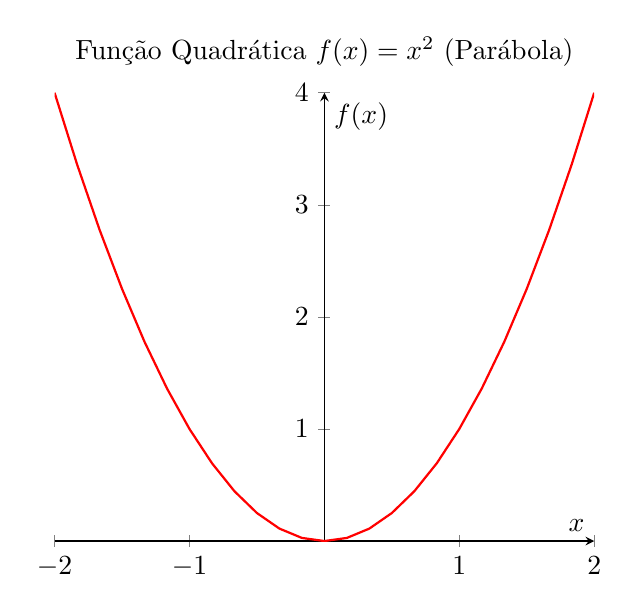
\begin{tikzpicture}
    \begin{axis}[
        title={Função Quadrática $f(x)=x^2$ (Parábola)},
        axis lines=middle,
        xlabel={$x$},
        ylabel={$f(x)$},
        xmin=-2, xmax=2, ymin=0, ymax=4]
    \addplot[red, thick, domain=-2:2] {x^2};
    \end{axis}
    \end{tikzpicture}
    \caption{Gráfico de uma função quadrática $f(x)=x^2$, representando uma parábola.}
    \label{fig:funcao_quadratica}
\end{figure}
% -----------------------------------------------





\newpage % Nova Página 
% -----------------------------------------------
\section{Exemplo de Lista de Tabelas}
% -----------------------------------------------

\noindent Esta seção demonstra a correta formatação ABNT para tabelas e garante o preenchimento da Lista de Tabelas.

% -----------------------------------------------
\begin{table}[H]
    \centering
    \caption{Recursos Utilizados por Componente}
    \label{tab:recursos_comp}
    \begin{tabular}{lrr}
        \toprule
        Componente & RAM (MB) & CPU (\%) \\
        \midrule
        Backend API & 512 & 30 \\
        Frontend UI & 128 & 15 \\
        \bottomrule
    \end{tabular}
\end{table}

\begin{table}[H]
    \centering
    \caption{Comparativo de Linguagens de Programação}
    \label{tab:linguagens_comp}
    \begin{tabular}{ccc}
        \toprule
        Linguagem & Desempenho & Curva de Aprendizado \\
        \midrule
        Python & Médio & Baixa \\
        C++ & Alta & Alta \\
        \bottomrule
    \end{tabular}
\end{table}
% -----------------------------------------------


\chapter{Suspendisse vel felis}
\lipsum[121]

\section{Curabitur et nunc}
\lipsum[8] % Gera texto de exemplo para preencher a página. 

\subsection{Curabitur dictum gravida}
\lipsum[5]

\subsubsection{Curabitur nunc}
\lipsum[6]

\subsubsubsection{Vestibulum luctus}
\lipsum[111]





\chapter{Morbi Suspendisse Praesent}

\section{Nullam at lectus}
\lipsum[10] % Gera texto de exemplo para preencher a página. 
\subsection{Nullam at lectus}
\lipsum[11] % Gera texto de exemplo para preencher a página. 


\section{Praesent pretium}
\lipsum[12] % Gera texto de exemplo para preencher a página. 


% -----------------------------------------------
% Finaliza a parte no bookmark do PDF
% para que se inicie o bookmark na raiz
% e adiciona espaço de parte no Sumário
% -----------------------------------------------
\phantompart


% -----------------------------------------------
% ----------------Conclusão----------------------
% -----------------------------------------------
\chapter*[Considerações Finais]{Considerações Finais}
\addcontentsline{toc}{chapter}{CONSIDERAÇÕES FINAIS}
\lipsum[150] % Gera texto de exemplo para preencher a página.


% -----------------------------------------------
% -----------ELEMENTOS PÓS-TEXTUAIS--------------
% -----------------------------------------------
\postextual


% -----------------------------------------------
% ----------Referências bibliográficas-----------
% -----------------------------------------------
\chapter*{Referências}                                               % Insere o título
\markboth{Referências}{Referências}                                  % Título "Referências" no cabeçalho.
\addtocontents{toc}{\protect\vspace{\baselineskip}}                  % Adiciona uma linha.
\addcontentsline{toc}{chapter}{\protect\MakeUppercase{REFERÊNCIAS}}  % Nível 'chapter' para linha grossos.
\printbibliography[heading=none]                                     % Imprime a bibliografia.
% -----------------------------------------------


% -----------------------------------------------
% -----------------APÊNDICE---------------------- 
% -----------------------------------------------
\begin{apendicesenv}
\partapendices % Imprime uma página indicando o início dos apêndices

\chapter{Quisque libero justo}

\section{Aliquam viverra arcu}
\lipsum[140] % Gera texto de exemplo para preencher a página. 

\section{Mauris consequat}
\lipsum[120] % Gera texto de exemplo para preencher a página. 
\end{apendicesenv}
% -----------------------------------------------


% -----------------------------------------------
% ------------------ANEXOS-----------------------
% -----------------------------------------------
\begin{anexosenv}
\partanexos % Imprime uma página indicando o início dos anexos

\chapter{Morbi ultrices rutrum lorem}

\section{Pellentesque sodales}
\lipsum[40] % Gera texto de exemplo para preencher a página. 

\section{Curabitur diam tortor}
\lipsum[54] % Gera texto de exemplo para preencher a página. 
\end{anexosenv}
% -----------------------------------------------

\end{document} 